\cleardoublepage
\chapter{Introduction}
%\label{ch:chapter1}
\label{makereference}

\section{Motivation and objectives}

La exploración espacial cumple muchos objetivos, siendo el más obvio recopilar información acerca de nuestro planeta y lo que le rodea. Para ello se crean sensores capaces de recopilar información, como por ejemplo antenas o telescopios que son usados tanto desde la Tierra como enviados a bordo de naves espaciales. Uno de ellos son las cámaras hiperespectrales, que toman fotos en cientos de bandas distintas. Estos datos permiten encontrar objetos, detectar materiales o identificar procesos. A medida que la tecnología avanza, estos sensores evolucionan requiriendo de soluciones de procesado acordes para interpretar los datos o comprimirlos y enviarlos a tierra.
\\
\\
El objetivo de este trabajo es la implementación de uno de estos algoritmos de forma que resulte preferente el procesado en la aeronave frente a la transmisión de los datos crudos.
\\
Para ello se evaluarán diferentes algoritmos y se escogerá una plataforma hardware. Se realizará una primera implementación del algoritmo en punto flotante y se estudiará su transformación a aritmética de enteros. Este paso es necesario ya que el mayor impedimento de estos algoritmos para ser implementados en hardware es el alto número y complejidad de sus operaciones. Con la aritmética bien definida, se adaptará su implementación y se hará una comparación de precisión y rendimiento entre la primera versión en punto flotante y la versión entera.

\section{Related work}
En este apartado se va a realizar una revisión del estado del arte sobre el uso de FPGAs en aplicaciones espaciales en general y de implementaciones relacionadas con el algoritmo desarrollado en este trabajo.
\\
\\
En \cite{lopez_promise_2013} se realiza un estudio sobre la situación actual del uso de FPGA a bordo de aeronaves para análisis hiperespectrales y se presentan implementaciones de dos algoritmos, ISRA y N-FINDR. Los resultados muestran numerosas ventajas de las FPGA frente a otro tipo de soluciones como GPUs como pueden ser su menor tamaño y peso y su resistencia frente a radiación. Además se recalca su capacidad de reconfiguración incluso después del lanzamiento del sistema.
\\
\\
En \cite{gonzalez_fpga_2016} se presenta una implementación de un algoritmo de generación de objetivos. Se usa un inversor por el método de eliminación de Gauss Jordan al igual que en este trabajo y los resultados se presentan sobre la misma plataforma.
\\
\\
En \cite{colome_garcia_implementacion_2013} se realiza un estudio del mismo algoritmo que se implementará en este trabajo sobre una FPGA. El resultado es positivo con una reducción del tiempo de cálculo frente a soluciones basadas en software. Sin embargo, este estudio se realizó solo sobre una implementación en punto flotante lo que lo limitó al procesado de imágenes hiperespectrales previamente reducidas dimensionalmente.
\\
\\
En \cite{theiler_onboard_2018} se propone el procesado de los datos a bordo con el objetivo de reducir el uso de red y acelerar el procesamiento de los datos. Uno de los pasos de este procesado es también el algoritmo RX que se implementará en este trabajo.
\\
\\
En general, los trabajos anteriores presentan buenos resultados sobre estos sistemas y expectativas a un aumento de uso, motivado por sistemas de captura de imágenes cada vez mas avanzados que llevan el hardware a sus limites.

\subsection{Reconfigurable hardware}
Las FPGA (de sus siglas en inglés, field programmable gate arrays) son chips basados en una matriz de bloques configurables llamados CLB (del ingles, configurable logic block) interconectados a su vez por una red también configurable \ref{fig:clb}.

\begin{figure}[h!]
\centering
\includegraphics[height=2.6in]{figures/clb.png}
\caption{Generic FPGA hardware architecture. Depicted is the basic structure of a CLB and the interconnecting network.}
  \label{fig:clb}
\end{figure}

\pagebreak

Al contrario que sistemas de propósito general como CPUs o GPUs, está arquitectura permite diseñar algoritmos con anchos de cálculo arbitrarios, lo que resulta en muy buen rendimiento a la hora de procesar imágenes, tanto energético como temporal \ref{fig:op_watt}.

\begin{figure}[h!]
\centering
\includegraphics[height=1.8in]{figures/op_watt.png}
\caption{In image analysis kernels  such  as  lookuptable, histogram, and histogram equalization, the energy/frameconsumption  of  the  FPGA  achieves  an  average  reduction  of 1.2× compared  to  the  GPU.  For  kernels  with  more branching  conditions  and  complex  memory  access  patterns, such as integral image, mean/std, and min/max locations, the FPGA’s  implementation  achieved  an  average  reduction  ratioof 3.5× compared to the GPU\cite{ochoa-ruiz_high-level_2012}}
  \label{fig:op_watt}
\end{figure}

\pagebreak

El entorno espacial no solo limita las capacidades energéticas, también presenta un desafío de cara a la radiación ionizante. Al ser este uno de los mercados objetivo de los fabricantes de FPGA, existen numerosos chips con las certificaciones de resistencia a radiación necesarias.
%http://microelectronics.esa.int/techno/fpga_002_01-0-4.pdf
%https://amstel.estec.esa.int/tecedm/website/biblio/AFLDCIS2010.pdf
\\
Las ASICs proporcionan la misma flexibilidad que las FPGA a la hora del diseño pero su rigidez a la hora de fabricación les permite lograr un mejor rendimiento al solo incluir la lógica especifica del diseño, sin embargo, su coste en provectos de pequeña a mediana escala resulta prohibitivo. Además, la flexibilidad de las FPGA permite la reconfiguración ya en la nave, permitiendo el uso de diferentes algoritmos o el parcheo de bugs.
%https://iopscience.iop.org/article/10.1088/1742-6596/1195/1/012012/pdf
%https://amstel.estec.esa.int/tecedm/website/stag_ygt/Boada.pdf
\\
\\
Además, puesto que la mayoría de algoritmos comparten ciertas operaciones básicas como pueden ser almacenamiento u operaciones matemáticas de precisión alta, los fabricantes de FPGA incluyen ciertos bloques prefabricados en el circuito, que aunque quitan cierta flexibilidad proporcionan mejor rendimiento que la misma lógica en CLBs. Estos bloques son principalmente memorias RAM y DSPs que permiten variedad de operaciones, entre ellas multiplicaciones o acumulaciones. Esta arquitectura heterogénea \ref{fig:heterogenea} permite implementar algoritmos de alto rendimiento donde sería imposible usando solo lógica y acercan las FPGA un poco al ámbito de las ASIC\cite{zhou_efficient_2013}.
\\
\begin{figure}[h!]
\centering
\includegraphics[height=2.5in]{figures/FPGA_heterogenea.png}
\caption{3: Heterogeneous FPGA platform, depicting general configurable resources, DSPs, BRAMs and soft (implemented in logic) and hard (prefabricated) CPUs}
  \label{fig:heterogenea}
\end{figure}
\\

\subsection{Hyperspectral imagery}
Una cámara de fotos estándar permite capturar imágenes compuestas de 3 bandas de luz diferenciadas, que los humanos percibimos como rojo, verde y azul. Sus espectros corresponden con altas longitudes de onda entre $564$ y $580 nm$ para el rojo, medias  entre $534$ y $545 nm$ para el verde y cortas entre $420$ y $440 nm$ para el azul. El resto de espectros resultan invisibles para nuestra vista.
\\
Sin embargo, las cámaras hiperespecrales capturan información en muchos más espectros, tanto entre las bandas visibles como fuera de ellas permitiendo analizar un espectro mucho más amplio. Estas bandas suelen mostrarse como una tercera dimensión, dando el nombre de hipercubo a estás imágenes \ref{fig:cube}.
\\
\\
\begin{figure}[h!]
\centering
\includegraphics[height=2in]{figures/rgb_vs_hsi.jpeg}
\caption{Comparison between the three bands of a standard camera and the multiple bands of an hiperspectral camera}
  \label{fig:cube}
\end{figure}
\\
%url{https://towardsdatascience.com/what-are-hyper-spectral-images-a5de5d9fa91}
\\
\\
Estos espectros o bandas forman en su conjunto una firma hiperespectral para cada material, que al ser comparado con imágenes aéreas permiten reconocer diferentes tipos de vegetación, depósitos minerales o contaminantes sobre la corteza terrestre \ref{fig:cuprite}.
\\
\\
\begin{figure}[h!]
\centering
\includegraphics[height=6in]{figures/cuprite.png}
\caption{The map shown is a mineral map from an AVIRIS scene flown over Cuprite, Nevada, in 1995 \citep{noauthor_aviris_nodate}. It shows the mapping of many different minerals}
  \label{fig:cuprite}
\end{figure}
\clearpage


En este tipo de imágenes podemos hablar de dos tipos de resoluciones: espacial y espectral, siendo esta última única en este tipo de cámaras. Espacial se refiere a la cantidad de metros cubiertos por cada pixel, por lo que para una misma cámara podrá cambiar de una imagen a otra. La resolución espectral se refiere a la separación entre diferentes longitudes de onda medidos en un rango determinado, es decir cuantas mas bandas capturadas en un rango menor, mayor será la resolución espectral\cite{amigo_chapter_2020}.
\\

Conforme al avance de la tecnología, estas resoluciones siguen aumentando realzando la necesidad de sistemas de procesado acorde.

\subsection{Anomaly detection}
En teoría, un material debería tener siempre la misma firma espectral. En la práctica, la firma capturada nunca va a ser la misma que la medida en un laboratorio a causa de diferencias en la iluminación, efectos atmosféricos, ruido etc. resultando en variedad espectral para materiales similares\cite{borsoi_spectral_2020}.

Esto ha llevado al desarrollo de algoritmos que en vez de clasificar observaciones según su firma, buscan clasificar las observaciones entre materiales inusuales o anómalos y el fondo. Para ello se asume que el material -el objetivo- es espectralmente diferenciable del fondo. El fondo es derivado globalmente de la imagen asumiendo que sigue una distribución normal.

%\url{http://downloads.hindawi.com/journals/jece/2012/425947.pdf}\\
%\url{http://downloads.hindawi.com/journals/jece/2012/628479.pdf}\\
%\url{http://downloads.hindawi.com/journals/jece/2012/103286.pdf}\\
%\url{http://downloads.hindawi.com/journals/jece/2012/162106.pdf}

\subsubsection{RX algorithm}
El algoritmo Reed-Xiaoli detector de anomalías es un algoritmo común que sirve de base a muchos otros.%\url{http://downloads.hindawi.com/journals/jece/2012/162106.pdf}\url{http://downloads.hindawi.com/journals/jece/2012/425947.pdf}\\%https://www.researchgate.net/publication/224166337_A_tutorial_overview_of_anomaly_detection_in_hyperspectral_images
%\url{http://downloads.hindawi.com/journals/jece/2012/162106.pdf}

El algoritmo esta definido por la siguiente expresión\citep{molero_fast_2011}:
\\
\[\delta ^{RX}(x) = (x-\mu)^{T}K^{-1}(x-\mu)\]

\paragraph{}
\phantomsection
\label{mayor}
Donde $x$ es un pixel hiperespectral (un vector de tamaño igual al número de bandas), $\mu$ es la media de cada banda y $K$ es la matriz de covarianzas. Es importante decir que los resultados generados por el algoritmo son imágenes en escala de grises. Las anomalías poseen un valor alto, así, la primera anomalía corresponde con el pixel con el valor más alto, y así sucesivamente.

\subsubsection{Other methods}
Aparte del algoritmo RX, existen otros métodos para la detección de anomalías, aunque un número notable de ellos se basa en RX.

\subsubsection{Subspace methods}
Los métodos subspace son globales y aplican principal component analysis (PCA) o singular value decomposition (SVD) al hipercubo. Las primeras bandas de PCA/SVD son supuestas de ser el fondo y son eliminadas de diferente forma por cada método. No eliminar suficientes bandas implica que las anomalías pueden perderse entre el ruido del fondo y eliminar demasiadas que estas desaparecerían. La determinación del número correcto de bandas a eliminar sigue siendo objeto de estudio. \cite{borghys_hyperspectral_2012}

\paragraph{Subspace RX}
En este método, el algoritmo RX es aplicado sobre un número limitado de bandas PCA. Las primeras componentes son descartadas.

\paragraph{RX after orthogonal subspace projection}
En este método, las primeras componentes PCA/SVD definen el subespacio del fondo y los datos son proyectados sobre un espacio ortogonal antes de aplicar RX.

\paragraph{RX after partialling out the clutter subspace}
En este método, "the effect of the clutter" en un pixel es descartado por componentes al predecir cada uno de sus componentes espectrales como combinación lineal de sus componentes principales de alta varianza. Sobre los resultantes se aplica el algoritmo RX.

\paragraph{Complimentary subspace detector}
Este algoritmo no está basado en RX. En CSD, las componentes principales con mayor varianza son usadas para definir el subespacio del fondo y las demás PC para definir el subespacio del objetivo. El pixel es entonces proyectado sobre los dos subespacios y el resultado es la diferencia de estos.

\subsubsection{Local methods}
En los métodos locales el fondo es derivado de los pixeles vecinos o que rodean al pixel a testear (PUT). Se definen dos ventanas, una guard y una exterior, y los vecinos son los pixeles que se encuentran entre estas dos. A veces, por ejemplo en RX local se usa una tercera donde la covarianza del fondo es calculada en una ventana mayor que la media del fondo.
\paragraph{Quasi-local RX}
Quasi-local RX es un compromiso entre RX global y RX local, donde la matriz de covarianza global es decompuesta usando eigenvector/eigenvalues. Los eigenvectors son manetnidos, pero los eigenvalues reemplazados por la varianza local maxima, resultando en que las puntuaciones del detector serán menores en zonas con alta varianza.

\begin{figure}[h!]
\centering
%\includegraphics[height=2.5in]{figures/ventana.png}
\hspace*{100pt}%
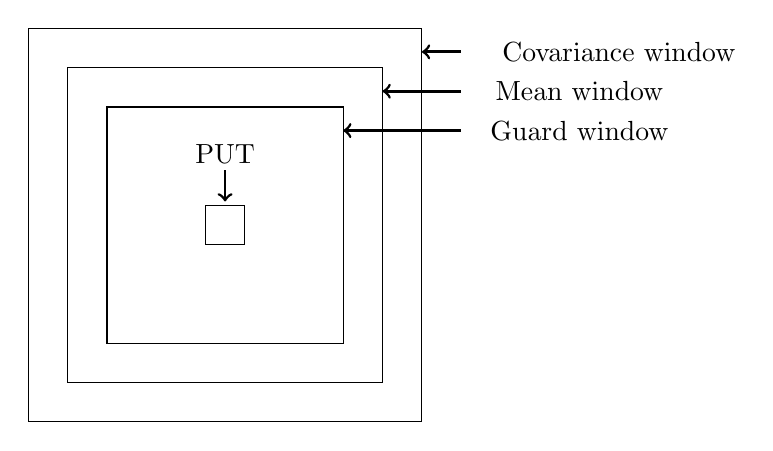
\begin{tikzpicture}
        \draw (0,0) rectangle (5,5);
        \draw[arrows=<-,line width=1pt](5,5-.3)--(5.5,5-.3);
        \draw (7.5,5-0.3) node{Covariance window};
        
        \draw (.5,.5) rectangle (4.5,4.5);
        \draw[arrows=<-,line width=1pt](4.5,4.5-.3)--(5.5,4.5-.3);
        \draw (7,4.5-0.3) node{Mean window};
        
        \draw (1,1) rectangle (4,4);
        \draw[arrows=<-,line width=1pt](4,4-.3)--(5.5,4-.3);
        \draw (7,4-0.3) node{Guard window};
        
        \draw (2.25,2.25) rectangle (2.75, 2.75);
        \draw[arrows=<-,line width=1pt](2.5, 3-.2)--(2.5, 3.2);
        \draw (2.5, 3.4) node{PUT};
    \end{tikzpicture}
\caption{Sliding triple window used in the local AD methods.}
  \label{fig:ventana}
\end{figure}

\subsubsection{Segmentation based methods}
En escenas complejas es difícil asumir que el fondo a a ser definido por una  distribución normal, por lo que se han desarrollado métodos que separan este en diferentes clases.
\paragraph{Class-Conditional RX}
En este método la imagen es primeramente segmentada y la matriz de covarianza y media calculada para cada una de estas clases. Los puntos corresponderán a la clase en la que su valor RX sea menor.

Existen más métodos dentro de los basados en segmentación, desde los que usan funciones estocásticas como Method Based on Multivariate Normal Mixture Models hasta métodos basados en Self-organizing maps.



\subsection{Comparing floating and fixed point}
\label{makereference}

En los sistemas informáticos, existen dos representaciones numéricas para números reales, punto fijo y flotante. Cuentan con diferentes aritméticas, lo que les otorga diferente rango y resolución con el mismo numero de bits. Por lo tanto, hay ciertas aplicaciones o plataformas mas afines a uno de ellos. Por ejemplo, la capacidad de los números de punto flotante de poder contener en la misma cantidad de bits tanto números muy grandes como muy pequeños y de ajustar su resolución acordemente resulta muy atractiva desde el punto de vista del programador pero la simpleza de las operaciones en punto fijo permiten su uso en microcontroladores de pequeño tamaño y el ahorro de recursos en FPGAs.%fuente
\begin{figure}[h!]
\centering
\includegraphics[height=2.5in]{figures/fp_vs_fp.png}
\caption{A FIR filter, originaly implemented as a single-precision floating-point filter and converted to fixed-point. The fixed-point design shows both resource reduction and latency improvements}
  \label{fig:fp}
\end{figure}
\\
Debido a la alta complejidad del análisis de imágenes hiperespectrales, las FPGA actuales tienen apenas capacidad para implementar algunos de estos algoritmos. Por lo tanto, uno de los objetivos de este trabajo es realizar dos implementaciones paralelas, una en punto flotante y otra en fijo y comparar sus resultados.

\pagebreak
\section{Project plan}
Primero se elegirá un algoritmo y un hardware sobre el que implementarlo. Deseablemente, este algoritmo debe ser conocido y encontrarse comúnmente en la literatura.
\\
Este algoritmo será implementado en software y esta implementación probada con imágenes reales contra software ya existente como ENVI o Spectral Python.
\\
Los pasos del algoritmo serán entonces optimizados para una arquitectura hardware y se estudiará la transformación del algoritmo de punto flotante a lógica de enteros o punto fijo.
\\
Esta transformación requiere decisiones de diseño que sacrifican precisión en pos de ahorrar recursos hardware, por lo que se tendrá que tener en cuenta el hardware subyacente.
\\
Posteriormente, se realizará una validación del diseño en hardware.
\\
Por último, se realizará un estudio sobre la precisión de los resultados obtenidos.
\\
\\
    \begin{figure}[h!]
    \begin{tikzpicture}
      \GanttHeader{\textwidth-0.6cm}{2ex}{3.5cm}{10}
      \Task{1}{Research algorithms}{0.5}{1}
      \Task{2}{Software impl.}{1}{4}
      \Task{3}{Model hardware}{2}{4.5}
      \Task{4}{Hardware impl.}{6}{2}
      \Task{5}{Test and validation}{7}{2}
      \Task{6}{Report results}{8.5}{1}

      %\arrowwhereboxesoverlap[thick,red,->]{1}{2}
      %\draw [blue,dashed,very thick,->] (2b) -- ++ (0.2,0) |- (4a);
\end{tikzpicture}
    \caption{Gantt diagram with an overview of months and tasks}
    \label{fig:gantt}
    \end{figure}
